\documentclass[border=4pt]{standalone}
\usepackage[sfdefault,lining]{FiraSans}
\usepackage[T1]{fontenc}
\usepackage{amsmath,amssymb}
\usepackage{tikz}
\usetikzlibrary{arrows.meta,positioning,calc}
\definecolor{gaC}{HTML}{2A78D6}\definecolor{tsC}{HTML}{EB6834}\definecolor{maC}{HTML}{1BAF7A}
\definecolor{ink}{HTML}{0B0B0B}\definecolor{ink2}{HTML}{52514E}\definecolor{muted}{HTML}{898781}
\definecolor{gridc}{HTML}{E1E0D9}\definecolor{addC}{HTML}{1BAF7A}\definecolor{remC}{HTML}{E34948}
\begin{document}
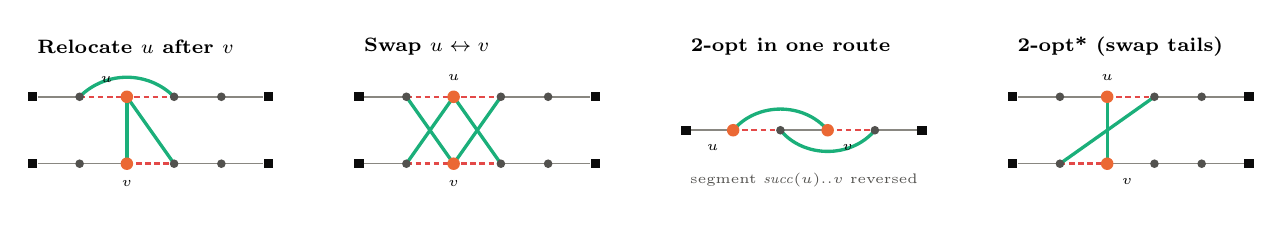
\begin{tikzpicture}[x=0.6cm,y=0.85cm,font=\scriptsize,
  c/.style={circle,fill=ink2,inner sep=1.1pt}, uv/.style={circle,fill=tsC,inner sep=1.6pt},
  dep/.style={rectangle,fill=ink,inner sep=1.7pt},
  old/.style={draw=remC,line width=0.9pt,dash pattern=on 2pt off 1.3pt},
  new/.style={draw=addC,line width=1.2pt}, keep/.style={draw=muted,line width=0.55pt}]
% ---------- generic helpers: a row = depot, 4 nodes, depot
\newcommand{\rowpts}[2]{% #1 = y, #2 = prefix
  \node[dep] (#2D0) at (0,#1) {}; \node[dep] (#2D5) at (5,#1) {};
  \foreach \k in {1,...,4} \coordinate (#2\k) at (\k,#1);}
% ---------- Relocate
\begin{scope}
  \node[font=\scriptsize\bfseries,anchor=west] at (-0.1,1.75) {Relocate $u$ after $v$};
  \rowpts{1}{A}\rowpts{0}{B}
  \draw[keep] (AD0)--(A1); \draw[keep] (A3)--(A4)--(AD5); \draw[old] (A1)--(A2)--(A3); \draw[new] (A1) to[bend left=45] (A3);
  \draw[keep] (BD0)--(B1)--(B2); \draw[old] (B2)--(B3); \draw[keep] (B3)--(B4)--(BD5);
  \draw[new] (A2)--(B2); \draw[new] (A2)--(B3);
  \foreach \k in {1,3,4} {\node[c] at (A\k) {}; \node[c] at (B\k) {};}
  \node[uv,label={[font=\tiny]above left:$u$}] at (A2) {}; \node[uv,label={[font=\tiny]below:$v$}] at (B2) {};
\end{scope}
% ---------- Swap
\begin{scope}[xshift=4.15cm]
  \node[font=\scriptsize\bfseries,anchor=west] at (-0.1,1.75) {Swap $u\leftrightarrow v$};
  \rowpts{1}{A}\rowpts{0}{B}
  \draw[keep] (AD0)--(A1); \draw[keep] (A3)--(A4)--(AD5); \draw[old] (A1)--(A2)--(A3);
  \draw[keep] (BD0)--(B1); \draw[keep] (B3)--(B4)--(BD5); \draw[old] (B1)--(B2)--(B3);
  \draw[new] (A1)--(B2)--(A3); \draw[new] (B1)--(A2)--(B3);
  \foreach \k in {1,3,4} {\node[c] at (A\k) {}; \node[c] at (B\k) {};}
  \node[uv,label={[font=\tiny]above:$u$}] at (A2) {}; \node[uv,label={[font=\tiny]below:$v$}] at (B2) {};
\end{scope}
% ---------- 2-opt
\begin{scope}[xshift=8.3cm]
  \node[font=\scriptsize\bfseries,anchor=west] at (-0.1,1.75) {2-opt in one route};
  \rowpts{0.5}{A}
  \draw[keep] (AD0)--(A1); \draw[old] (A1)--(A2); \draw[keep] (A2)--(A3); \draw[old] (A3)--(A4); \draw[keep] (A4)--(AD5);
  \draw[new] (A1) to[bend left=50] (A3); \draw[new] (A2) to[bend right=50] (A4);
  \foreach \k in {2,4} \node[c] at (A\k) {};
  \node[uv,label={[font=\tiny]below left:$u$}] at (A1) {}; \node[uv,label={[font=\tiny]below right:$v$}] at (A3) {};
  \node[font=\tiny,ink2] at (2.5,-0.25) {segment $\mathit{succ}(u)..v$ reversed};
\end{scope}
% ---------- 2-opt*
\begin{scope}[xshift=12.45cm]
  \node[font=\scriptsize\bfseries,anchor=west] at (-0.1,1.75) {2-opt* (swap tails)};
  \rowpts{1}{A}\rowpts{0}{B}
  \draw[keep] (AD0)--(A1)--(A2); \draw[old] (A2)--(A3); \draw[keep] (A3)--(A4)--(AD5);
  \draw[keep] (BD0)--(B1); \draw[old] (B1)--(B2); \draw[keep] (B2)--(B3)--(B4)--(BD5);
  \draw[new] (A2)--(B2); \draw[new] (B1)--(A3);
  \foreach \k in {1,3,4} \node[c] at (A\k) {}; \foreach \k in {1,3,4} \node[c] at (B\k) {};
  \node[uv,label={[font=\tiny]above:$u$}] at (A2) {}; \node[uv,label={[font=\tiny]below right:$v$}] at (B2) {};
\end{scope}
\end{tikzpicture}
\end{document}
